\documentclass[11pt,a4paper]{article}

%
% $Id: userguide.tex 526 2007-10-31 08:57:09Z schnelle $
%

\usepackage[latin1]{inputenc}
\usepackage{graphics}
\usepackage{graphicx}
\usepackage{url}
\usepackage{listings}
\usepackage{xcolor}
\usepackage{../jvoicexml}

\title{JVoiceXML 0.6 User Guide}
\version{0.6}
\author{Dirk Schnelle}
\email{dirk.schnelle@jvoicexml.org}

\date{}

\begin{document}
\pagestyle{empty}
\lstset{language=Java,language=XML,
        backgroundcolor=\color{lightgray},
        basicstyle=\small,
        numbers=left,
        numberstyle=\tiny,
        stepnumber=5}

\maketitle

\pagestyle{headings}

\tableofcontents

\newpage

\begin{abstract}
This documents describes the API of JVoiceXML from the user's point of
view. It provides information about the coding of clients for
the JVoiceXML voice browser.
\end{abstract}


\section{Introduction}
\label{sec:introduction}

JVoiceXML is a free VoiceXML~\cite{w3.org:voicexml} implementation written in 
the JAVA programming language. It offers a library for easy VoiceXML
document creation and a VoiceXML interpreter to process 
VoiceXML documents using JAVA standard APIs such as JSAPI~\cite{sun:jsapi} and
JTAPI~\cite{sun:jsapi}.

VoiceXML is hosted at SourceForge~\cite{sourceforge} as an open source project.
You find everything that is related to this project under
\url{http://sourceforge.net/projects/jvoicexml/}.
The work on the browser is still in progress and not all tags are
supported. You are invited to help us finishing the work to make this
project a success.

This document provides information about the installation and
configuration of the JVoiceXML voice browser and how to write
VoiceXML applications for this browser.
It is assumed that readers are familiar with the concepts of
VoiceXML and Java programming.

This document refers to UNIX and Windows systems. JVoiceXML will work 
any other operating systems that support Java 5, too.

Nobody is perfect, so you may find some errors or small things to correct.
Please let me know if you think you found something that should be written
differently or should be added.

\section{Architectural Overview}
\label{sec:arch-overv}

Before going into detail, the general architecture and concepts are presented.
The basic architecture is shown in figure~\ref{fig:architecture}.

\begin{figure}
\label{fig:architecture}
\caption{Basic architecture}
\begin{center}
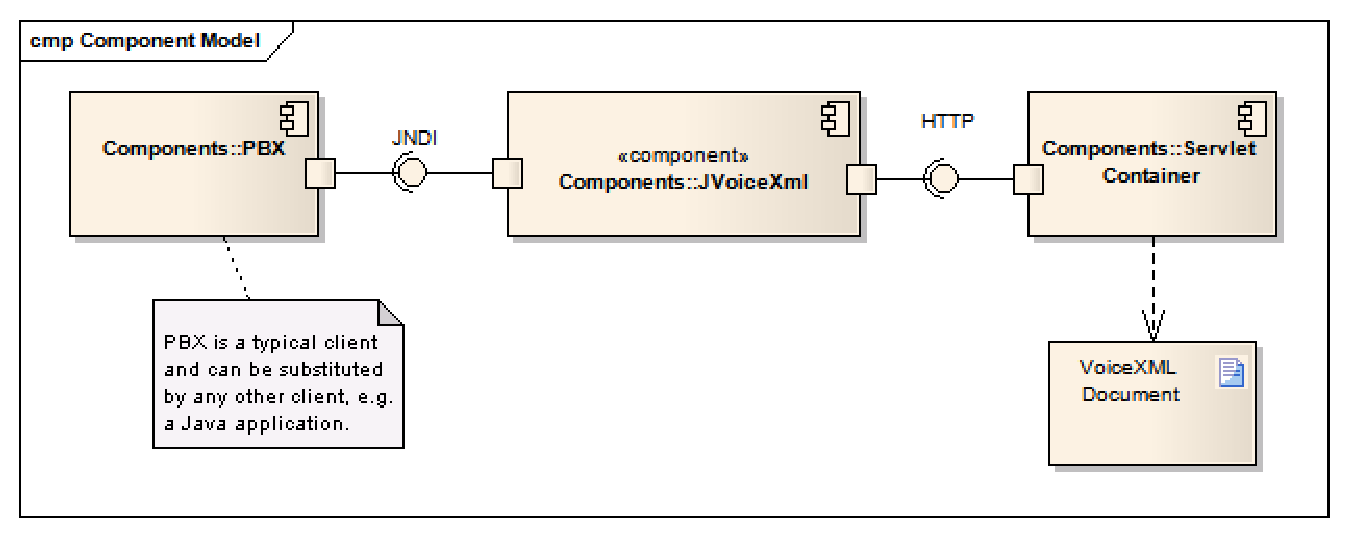
\includegraphics[scale=0.3]{architecture.eps}
\end{center}
\end{figure}

The VoiceXML documents are stored in a web server or a servlet container
and are accessed, e.g., via the HTTP protocol.
JVoiceXML runs as a standalone server and retrieves the documents from
the servlet container. 

Clients use the Java Naming and Directory Interface (JNDI)~\cite{sun:jndi} to 
access JVoiceXML. They can also initiate calls for an application using this 
technology. Currently there is no telephony support, but users can call 
applications from their own Java programs. How this is done is described in the 
following sections.

Conceptually JNDI allows to connect to a centralized running JVoice\-XML 
server. However this does not make much sense for the current demo 
implementation, since the speaker and the microphone of the JVoiceXML server
is used for speech output and input.

\section{Required Software}
\label{sec:required-software}

JVoiceXML is written in JAVA and you will at least need a JAVA compiler, an 
editor or preferably a JAVA IDE, see section~\ref{sec:ide}, and ANT, see 
section~\ref{sec:ant}, to run the browser and build the binaries for the 
clients. Tomcat from the Apache Jakarta project can be used as a servlet
container.

\subsection{IDE}
\label{sec:ide}

You can use the IDE of your choice to edit the sources and compile the 
demos. You can even use a simple text editor to perform this job.
Nevertheless there are some restriction that you cannot work around.

Your IDE must support at least J2SE 1.5. The demos use ANT 1.7 for compilation. 
ANT is not required but used as a means of IDE independent project setup.

\subsection{JAVA}
\label{sec:java}

Parts of the code of JVoiceXML are using features from the JAVA 5 API, so that
you will need at least J2SE 1.5 to compile the code. You can download it
for free from \url{http://java.sun.com/j2se/1.5.0/download.jsp}.

\subsection{ANT}
\label{sec:ant}

The demos are being built by an ANT build file It is recommended that
you use at least ANT 1.7.0. 
If you don't have ANT installed, you can download the current release
from \url{http://ant.apache.org}.

Nearly all IDEs feature an ANT integration. This allows to use
your favorite IDE.

\subsection{Tomcat}
\label{sec:tomcat}

VoiceXML is designed to access documents via the HTTP protocol.
This guide uses Tomcat for this purpose. Tomcat can be obtained
from \url{http://jakarta.apache.org/tomcat}. You can also use
the servlet container of your choice.

\section{Installation}

You can download the compiled voice browser as \texttt{jvxml-VERSION.zip} from 
\url{http://jvoicexml.sourceforge.net/downloads.htm}.
\texttt{VERSION} has to be replaced by the used version number, i.e. 0.5.
Unpack the zipped distribution file and open a command prompt in that
directory. Call the installer 

\begin{lstlisting}
java -jar jvxml-VERSION-install.jar
\end{lstlisting}

For windows this should also work, if you double-click the jar. 

This will install the browser into a directory of your choice. In the rest of 
this document this directory will be referred as JVOICE\-XML\_HOME.

\section{Starting the browser}

After the installation, the browser is ready to use. 
The \texttt{bin} folder contains the files to start the browser,
depending on your operating system.

\subsection{Linux}

The shell script \texttt{startup.sh} located in the \texttt{bin} folder
of your JVoiceXML installation can be used to start the browser.

It is written to work independent to the current folder. Simply call

\begin{lstlisting}
sh JVOICEXML_HOME/bin/startup.sh
\end{lstlisting}

After the start lots of debug information will be displayed.
It may take a while until the TTS engine and the recognizer are launched.
The voice browser can be used, if you see the message

\begin{lstlisting}
VoiceXML interpreter started.
\end{lstlisting}

\subsection{Windows}

The windows executable \texttt{JVoiceXML.exe} located in the \texttt{bin}
folder of your JVoiceXML installation can be used to start the browser.

This is simply a wrapped Java call and should also work with a double-click
in the windows explorer.

From The command line prompt, call

\begin{lstlisting}
JVOICEXML_HOME\bin\JVoiceXML.exe
\end{lstlisting}

If you start the browser from the windows explorer, a command prompt will open.
After the start lots of debug information will be displayed.
It may take a while until the TTS engine and the recognizer are launched.
The voice browser can be used, if you see the message

\begin{lstlisting}
VoiceXML interpreter started.
\end{lstlisting}

\section{Running the demos}

The browser comes with some demo programs. You'll find them in the
directory \texttt{JVOICEXML\_HOME/demo}. Use the IDE of your choice
and explore there contents. Some features of the browser can 
become more clear.

The demo programs feature an ANT script which can be used for starting.
Since they come from the development environment, there are some
properties, that need to be overwritten in the installed version.
To do that, create a file \texttt{jvoicexml.properties} in the
\texttt{JVOICEXML\_HOME} directory with the following contents

\begin{lstlisting}
3rdparty.dir=../../lib
log4j.lib.dir=../../lib
jvoicexml.lib.dir=../../lib
\end{lstlisting}

This tells the build scripts where to find the libraries that are required
to compile and run the demos.

In most cases it should be sufficient to change to each demo directory
and call

\begin{lstlisting}
ant run
\end{lstlisting}

This does not work for the \emph{HelloWorldServletDemo}. In this
case you have to add the location of \texttt{servlet-api.jar} to
the \texttt{jvoicexml.properties} by adjusting the property
\texttt{servlet.lib.dir}.

Before you can run this demo, call

\begin{lstlisting}
ant war
\end{lstlisting}

to create a war archive that must be deployed to you servlet container
before running the demo.

\section{A first example}

This first example shows, how VoiceXML documents are accessed from a
servlet container or a web server and how clients can start the application.

\subsection{Creating the VoiceXML file}
\label{sec:hello-vxml}

This first example is very simple, it just echos a 'hello world'.
Create a file \texttt{hello.vxml} with the following content:

\begin{lstlisting}[language=XML]
<?xml version="1.0" encoding="UTF-8"?> 
<vxml xmlns="http://www.w3.org/2001/vxml" version="2.1">
  <form>
    <block>Hello World!</block>
  </form>
</vxml>
\end{lstlisting}

Copy this file to a directory of your web server, that can be accessed
by a browser. For Tomcat create a directory \texttt{demo1} in
the \texttt{\$CATALINA\_HOME/web\-apps} directory and copy the VoiceXML
file to this directory. In order to make this
an accessible web application, create the empty sub-folder \texttt{WEB-INF}
in \texttt{demo1}.

Now try to access the file in your browser. For Tomcat, this is
\url{http://localhost:8080/demo1/hello.vxml}. If all went well, the
contents of this file is displayed in the browser. In some cases the file
might be offered for download. This is the default behaviour of your browser if
it can not determine the type of the file. Download the file in your
favourite editor and verify that this is your VoiceXML code.

\subsection{Writing the Client}

A client is a program that remotely calls JVoiceXML and initiates calls. Create 
a Java file \texttt{Demo1.java} with the following content:

\begin{lstlisting}[language=Java]
public class Demo1 {
    public static void main(String[] args) {
    }
}
\end{lstlisting}

First, we need to connect to the JVoiceXML voice browser. JVoiceXML
uses JNDI over RMI~\cite{sun:rmi,sun:rmi_jndi} for this purpose. 
The following code snippet
shows, how to obtain a remote reference to the main entry for
all client applications \texttt{org.jvoicexml.JVoiceXml}:

\begin{lstlisting}[language=Java]
import javax.naming.Context;
import javax.naming.InitialContext;

import org.jvoicexml.JVoiceXml;
...
    public static void main(String[] args) {
        Context context;
        try {
            context = new InitialContext();
        } catch (javax.naming.NamingException ne) {
	    ne.printStackTrace();
            System.exit(-1);
        }

        JVoiceXml jvxml;
        try {
            jvxml = (JVoiceXml) context.lookup("JVoiceXml");
        } catch (javax.naming.NamingException ne) {
	    ne.printStackTrace();
            System.exit(-1);
    }
...
\end{lstlisting}

First, a \texttt{Context} is created to access JNDI resources.
The settings how to do this are obtained from a file named
\texttt{jndi.properties}, which is in the \texttt{CLASSPATH}.
\texttt{jndi.properties} has the following contents:

\begin{lstlisting}
java.naming.factory.initial=\
    com.sun.jndi.rmi.registry.RegistryContextFactory
java.naming.provider.url=rmi://localhost:1099
java.naming.rmi.security.manager=true
\end{lstlisting}

The location of JVoiceXML is stored in the property 
\texttt{java.naming.pro\-vider.url}. If you want to access JVoiceXML on a 
different computer you have to replace \texttt{localhost} with the IP address 
or name of that computer.

The classes  that are required to access JVoiceXML, like 
\texttt{org.jvoicexml.JVoiceXml}, are part of the
\texttt{jvxml-client.jar}, which can be found in the \texttt{lib}
folder of you JVoiceXML installation. This jar contains all classes, that you 
need to write client applications.

Next, we call the browser to process the application. This is done by creating 
a \texttt{org.jvoicexml.Session} object.

\begin{lstlisting}[language=Java]
...
import org.jvoicexml.Session;
...

    public static void main(String[] args) {
        ...
        JVoiceXml jvxml;
        try {
            jvxml = (JVoiceXml) context.lookup("JVoiceXml");
        } catch (javax.naming.NamingException ne) {
	    ne.printStackTrace();
            System.exit(-1);
    }

    final Session session = 
        jvxml.createSession(null);

    final URI uri;
    try {
        uri = 
          new URI("http://localhost:8080/demo1/hello.vxml");
    } catch (URISyntaxException e) {
        e.printStackTrace();

        System.exit(-1);
    }

    try {
        session.call(uri);

        session.waitSessionEnd();

        session.close();
    } catch (org.jvoicexml.event.JVoiceXMLEvent e) {
        e.printStackTrace();

        System.exit(-1);
    }
...
\end{lstlisting}

The argument on the \texttt{createSession} method must be 
\texttt{null}. It is reserved for future use, if we have telephony
support. The argument for \texttt{call} must point to to URI of the
root document of your application.

\subsection{Starting the Client}

The JNDI implementation of JVoiceXML is based on RMI, and
the implementation for the used interfaces are obtained by
RMI dynamic code download. This means that you have to provide
the location of the library with the implementation of the
interfaces and a security policy file.

For the start, this security policy file \texttt{jvoicexml.policy}
allows everything to the remote user:

\begin{lstlisting}
grant {
    permission java.security.AllPermission;
};
\end{lstlisting}

The location of the policy file and \texttt{jvxml.jar} are provided by the 
following environment properties

\begin{lstlisting}
-Djava.security.policy=jvoicexml.policy \
-Djava.rmi.server.codebase=\
    file://${JVOICEXML\_HOME}/lib/jvxml.jar
\end{lstlisting}

Note that the path to \texttt{jvxml.jar} must be hierarchical.

\section{Capturing User Input}

This example shows, how JVoiceXML can be used to capture user input. 

\subsection{Creating the VoiceXML file}

We use the same environment, as introduced in section~\ref{sec:hello-vxml}. Here
we use the source folder \texttt{demo2}.
The demo asks the user a question with the possible answers
\emph{Yes} and \emph{No}.

Our VoiceXML code in the file \texttt{input.vxml} looks like this:

\begin{lstlisting}[language=XML]
<?xml version="1.0" encoding="UTF-8"?> 
<vxml xmlns="http://www.w3.org/2001/vxml" version="2.1"
      xml:base="http://localhost:8080/demo2/">
  <form>
    <field name="answer">
      <grammar src="yesno.gram" type="application/x-jsgf"/>
      <block>Do you like this example?</block>
      <noinput>
        Please say something.
      </noinput>
      <nomatch>
        Please say yes or no.
      </nomatch>
      <filled>
        <if cond="answer=='yes'">
           You like this example.
        <else/>
           You do not like this example.
        </if>
      </filled>
    </field>
  </form>
</vxml>
\end{lstlisting}

\subsection{Creating the Grammar}

The VoiceXML code above relates to the grammar \texttt{yesno.gram}. At the
current state of development, JVoiceXML supports only grammars in JSGF format.
Others will come soon.

Create a file \texttt{yesno.gram} with the following content:

\begin{lstlisting}
grammar yesno;
public <yesno> =  yes | no

\end{lstlisting}

Add the grammar file to you war archive.

JVoiceXML is shipped with sphinx4 as a demo speech recognizer. Unfortunately,
the JSAPI interfaces seems to be buggy and it is not possible to dynamically
load or activate grammars. All grammars that are defined at start are active 
throughout the application. JVoiceXML does not have any limitations in that way.
You will be able to use grammar activation as it is meant to be, if you use your
own JSAPI compliant recognizer.

Now, edit the file \texttt{sphinx4.config.xml} and tell sphinx about your new 
grammar.

Look for the following code snippet

\begin{lstlisting}[language=XML]
<component name="jsgfGrammar" 
           type="edu.cmu.sphinx.jsapi.JSGFGrammar">
    <property name="dictionary" value="dictionary"/>
    <property name="grammarLocation"
         value="file:config/"/>
    <property name="grammarName" value="movies"/>
    <property name="logMath" value="logMath"/>
</component>
\end{lstlisting}

and replace \emph{movies} by \emph{yesno}.

Place a copy of the grammar file in the \texttt{\$JVOICE\-XML\_HOME/config}
folder, so that JVoiceXML is able to find it.

\begin{lstlisting}[language=XML]
<component name="jsgfGrammar" 
           type="edu.cmu.sphinx.jsapi.JSGFGrammar">
    <property name="dictionary" value="dictionary"/>
    <property name="grammarLocation"
         value="file:config/"/>
    <property name="grammarName" value="yesno"/>
    <property name="logMath" value="logMath"/>
</component>
\end{lstlisting}

Afterwards you will have to restart JVoiceXML.

\subsection{Writing the Client}

The client for this demo looks pretty much like the client for the \emph{Hello
World!} example.

Copy the file \texttt{Demo1.java} into a file \texttt{Demo2.java} and adapt the
URI to point to the demo2.

\begin{lstlisting}[language=Java]
...
import org.jvoicexml.Session;
...

    public static void main(String[] args) {
        ...
        JVoiceXml jvxml;
        try {
            jvxml = (JVoiceXml) context.lookup("JVoiceXml");
        } catch (javax.naming.NamingException ne) {
	    ne.printStackTrace();
            System.exit(-1);
    }

    final Session session = 
        jvxml.createSession(null);

    final URI uri;
    try {
        uri = 
          new URI("http://localhost:8080/demo2/input.vxml");
    } catch (URISyntaxException e) {
        e.printStackTrace();

        System.exit(-1);
    }

    try {
        session.call(uri);

        session.waitSessionEnd();

        session.close();
    } catch (org.jvoicexml.event.JVoiceXMLEvent e) {
        e.printStackTrace();

        System.exit(-1);
    }
...
\end{lstlisting}

\section{Configuration}

After the installation, JVoiceXML should run out of the box. However, there may 
be some circumstances, where it is necessary, to adapt the configuration.

\subsection{JNDI Port}

The remote access for clients is based on RMI, using the default RMI port. This
can conflict with other applications that also use this technology, like JBoss.

If you want to change the RMI port for JVoiceXML, you have to make changes in 
two configuration files that you can find in the folder 
\texttt{\$JVOICE\-XML\_HOME/config}.

In the file \texttt{jvoicexml.xml} you have to adapt the \texttt{port} 
attribute in following section

\begin{lstlisting}
<bean id="jndi" 
      class="org.jvoicexml.jndi.JVoiceXmlJndiSupport">
  <property name="registry">
    <bean id="registry"
      class="org.jvoicexml.jndi.JVoiceXmlRegistry">
      <property name="port" value="1099"/>
	</bean>
  </property>
</bean>
\end{lstlisting}

In addition you have to adapt the file \texttt{jndi.properties}.
Change the port to the same value as above.

\begin{lstlisting}
java.naming.provider.url=rmi://localhost:1099
\end{lstlisting}

\section*{Document history}

\begin{tabular}{|l|p{5cm}|l|l|}
\hline
\textbf{Version} & \textbf{Comment} & \textbf{Author} & \textbf{Date} \\
\hline
\hline
0.1 & Initial Release & Dirk Schnelle & 04/24/2006 \\
\hline
0.2 & First demo & Dirk Schnelle & 04/26/2006 \\
\hline
0.3 & Architectural overview & Dirk Schnelle & 04/27/2006 \\
\hline
0.4 & Running the demos & Dirk Schnelle & 07/20/2006 \\
\hline
0.4.1 & Adaption to refactoring of 0.5.5 & Dirk Schnelle & 03/07/2007 \\
\hline
0.5 & Started user input example & Dirk Schnelle & 03/13/2007 \\
\hline
\end{tabular}


\bibliography{userguide}
\bibliographystyle{plain}


\end{document}


% LocalWords:  backgroundcolor lightgray basicstyle numberstyle stepnumber API
% LocalWords:  JVoiceXML VoiceXML APIs JSAPI JTAPI SourceForge JVoice mkdir cd
% LocalWords:  jvxml startup TTS exe Schnelle userguide servlet http JNDI IDE
% LocalWords:  JVoiceXML IDE's vxml xml UTF xmlns webapps args RMI ne lookup
% LocalWords:  InitialContext printStackTrace JVoiceXml jndi CLASSPATH vider IP
% LocalWords:  url localhost ApplicationRegistry uri toURI mue urise jvxmle api
% LocalWords:  createApplication helloworldservlet createSession RMI's
% LocalWords:  jvoicexml HelloWorldServletDemo
